\hyt{slunecnyhrob}
\song{Slunečný hrob}

\intro{
	
\vspace{-30pt}
\hspace{21pt}
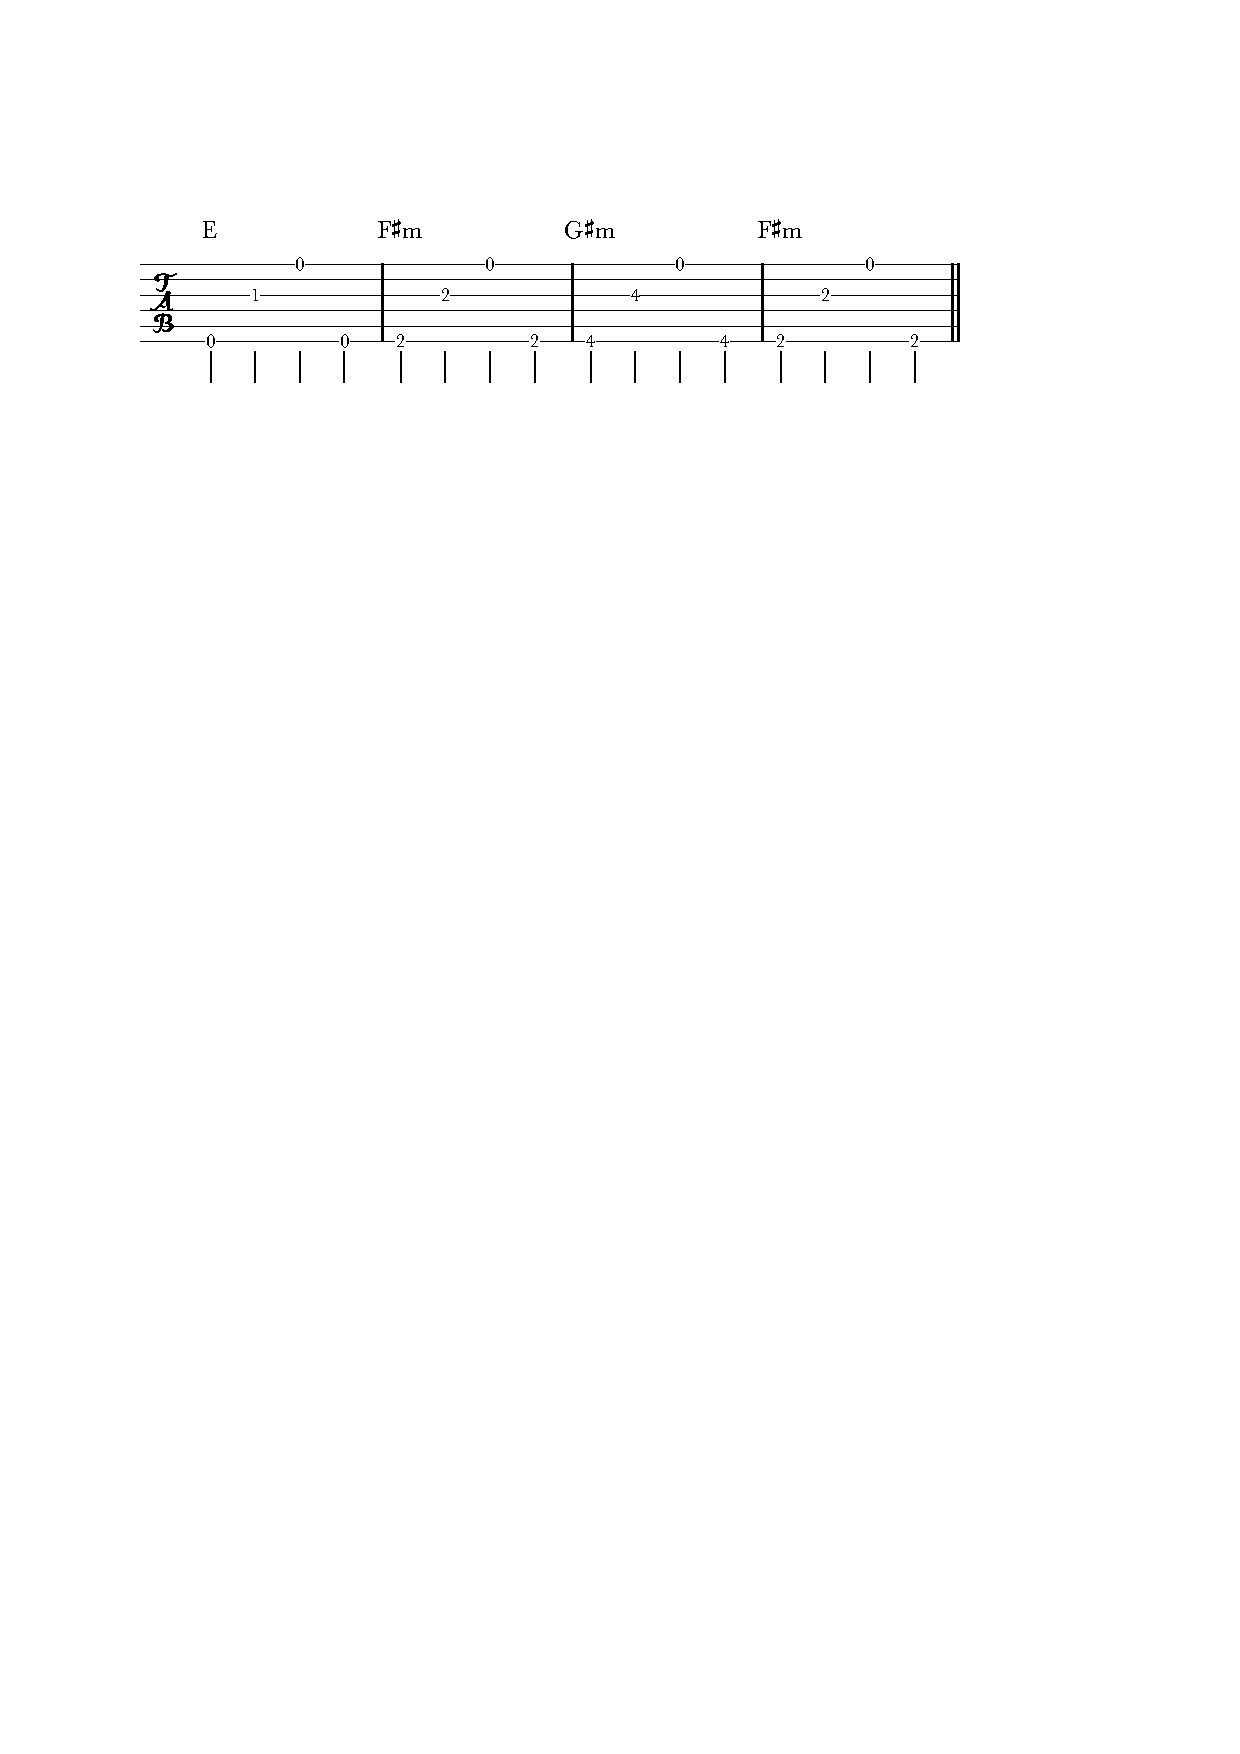
\includegraphics[width=0.7\linewidth]{scores/slunecnyhrob_intro.pdf}
}

\emph{rec:} Usínám a chtěl bych se vrátit o nějakej ten rok zpátky,\\
bejt zase klukem, kterej si rád hraje a který je s tebou.

\vers{1}{
\chord{E}Zdá se \chord{F\kk m}mi, \mm\chord{G\kk m}je to \mm\chord{F\kk m}moc let,\\
\chord{E}já byl \chord{F\kk m}kluk, \mm\chord{G\kk m}kterej \chord{F\kk m}chtěl\\
\chord{E}znáti \chord{F\kk m}svět, \mm\chord{G\kk m}s tebou \chord{F\kk m}jsem si \chord{E}hrál.
}

\solon{1}{
	
\vspace{-30pt}
\hspace{21pt}
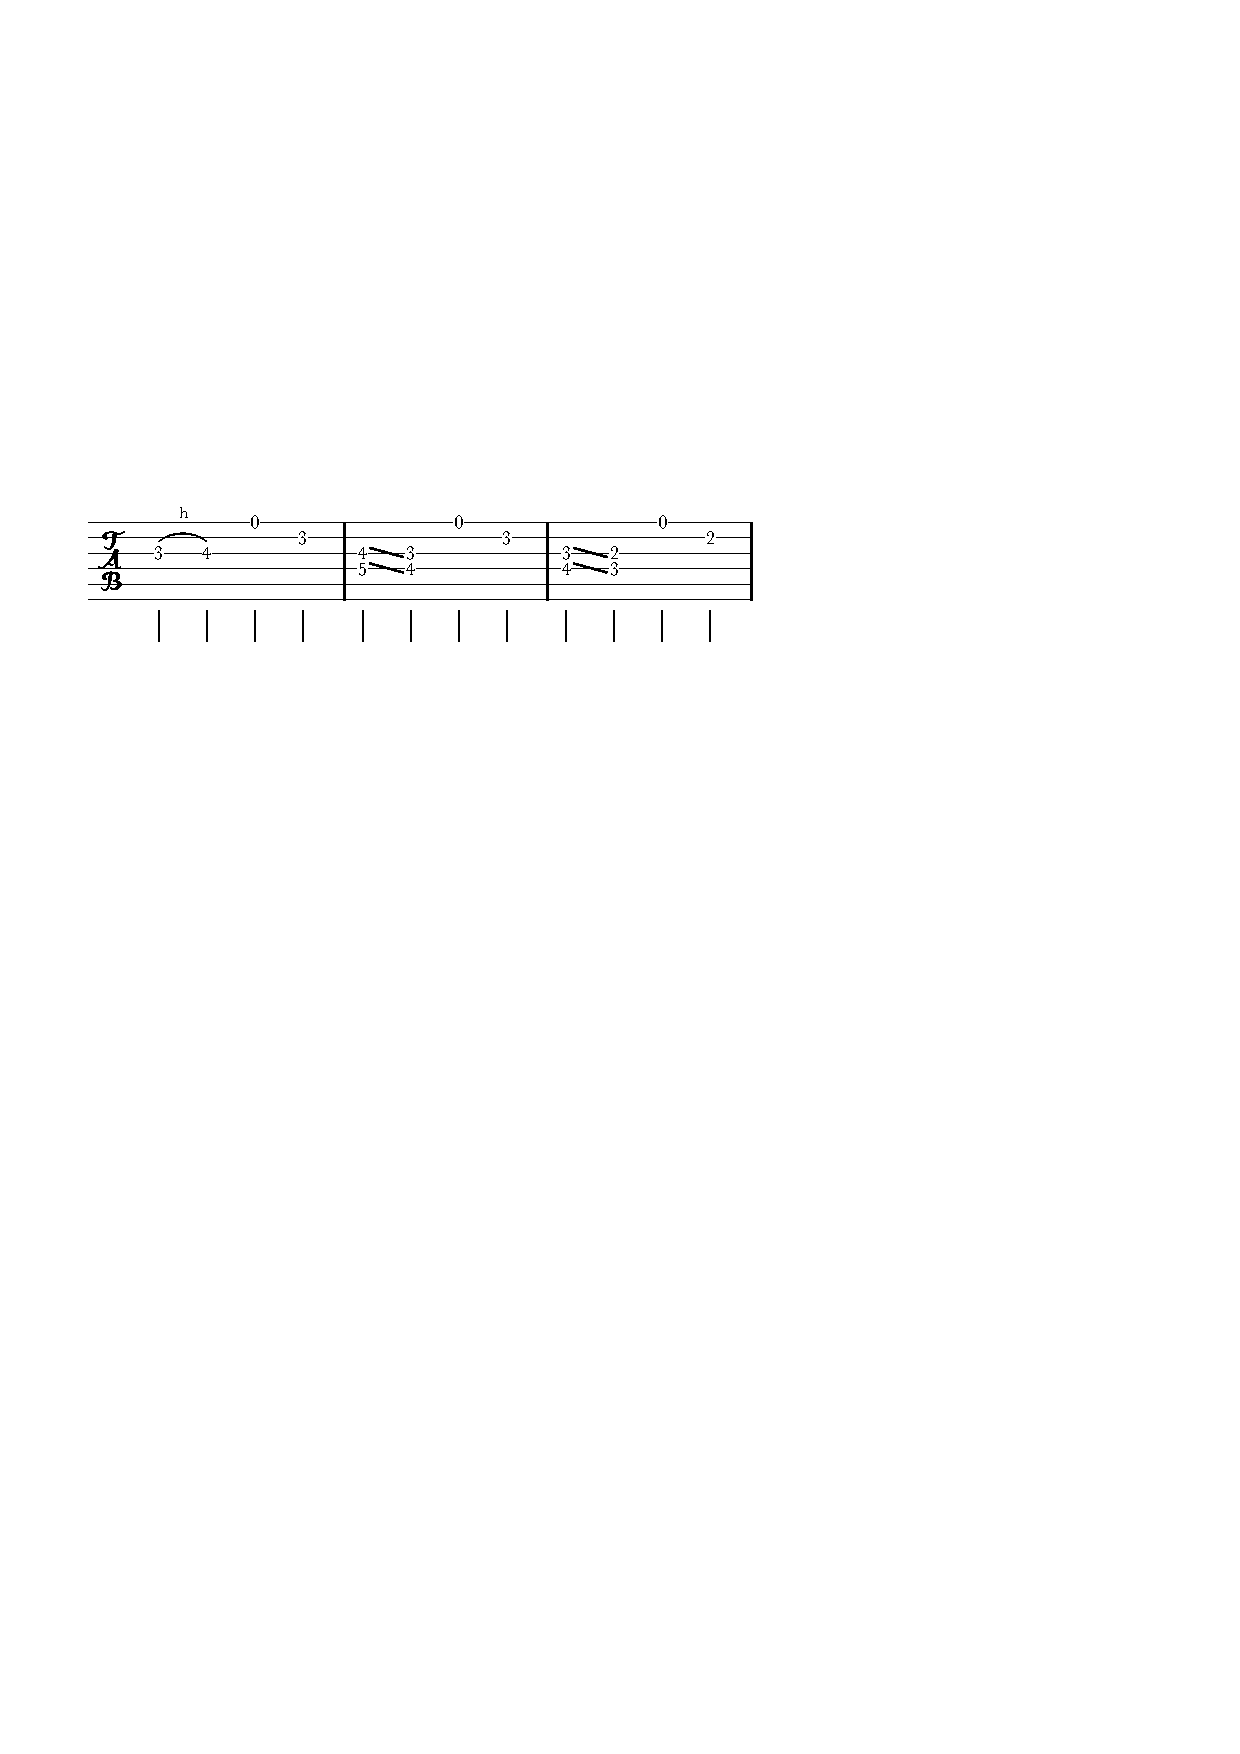
\includegraphics[width=0.7\linewidth]{scores/slunecnyhrob_solo.pdf}
}
\ns

\vers{2}{
Vrátím se a chtěl bych rád\\
být s tebou, zavzpomínat,\\
mám teď, ale zprávu zlou.
}

\refrain{
\chord{C\kk m}Su\nc\chord{D\kk m}chá \mm\chord{A}hlína \chord{G\kk m}\mm ta\mm\chord{F\kk m}dy,\\
bez kvítí, bez vody,\\
\chord{G\kk m}já na ni \chord{F\kk m}poklekám, \chord{G\kk m}vzpomínkou po\chord{H}cta se vzdává.
}

\vers{3}{
Loučím se a něco však tam zůstalo\\
z těch našich dnů\\
já teď vím, věrný zůstanu.
}\solosm{1}
\ns

\solon{2}{
\textit{akordy jako ve sloce}
} \refsm{}
\ns

\vers{4}{
=\mm \textbf{3.}
}\refsm{}
\vspace{2mm}


\emph{rec:} Nemohu spát, probouzím se a zase se nemohu ubránit myšlence\\
vrátit se o nějakej ten rok zpátky, bejt zase malým klukem,\\
který si rád hraje a který je s tebou.
\newpage
